\chapter{Marco Aplicativo: Servicio PAWARE}
\pagestyle{fancy}

Este capítulo introduce el contexto aplicativo del Trabajo Especial de Grado, enfocándose en la infraestructura de microservicios y observabilidad sobre la cual se implementa el modelo de auto-mantenimiento asistido por inteligencia artificial. Se describen los componentes del ecosistema, la estrategia de despliegue y gestión, el diseño e implementación del servicio PAWARE, los escenarios de prueba y los resultados obtenidos.

\section{Arquitectura del Ecosistema de Microservicios y Observabilidad}

Esta sección describe la infraestructura tecnológica sobre la cual se implementará el modelo de mantenimiento de software. Se detalla la migración del backend monolítico de PortalAsig a una arquitectura de microservicios, la incorporación de un robusto stack de observabilidad y el mecanismo de despliegue y gestión del entorno completo, tal como ha sido configurado y validado.

\subsection{Migración y Componentes del Backend}
El sistema PortalAsig, inicialmente concebido como un monolito, ha sido refactorizado hacia una arquitectura de microservicios. Este nuevo ecosistema se compone de múltiples nodos especializados desarrollados en Spring Boot, cada uno con responsabilidades bien definidas:
\begin{itemize}
    \item \textbf{Gestión de Identidad y Acceso:} Microservicio encargado de la autenticación, autorización y emisión de tokens seguros.
    \item \textbf{Gestor de Sitios Académicos:} Maneja la lógica de negocio central, incluyendo la persistencia de cursos, semestres y contenido académico.
    \item \textbf{Servicio de Notificaciones:} Responsable del procesamiento asíncrono y despacho de correos electrónicos.
    \item \textbf{PAWARE:} El servicio de control autonómico que implementa el ciclo de auto-mantenimiento.
\end{itemize}
\begin{center}
    \textit{[Placeholder: Diagrama de Arquitectura de Microservicios detallando las conexiones y bases de datos por servicio]}
\end{center}
La configuración de estos nodos se gestiona a través de un servidor de configuración centralizado (\textit{Config Server}), el cual resuelve propiedades desde un repositorio distribuido. Cada componente persiste sus datos de manera aislada en instancias dedicadas, asegurando alta disponibilidad.

\subsection{Stack de Observabilidad}
Para permitir que PAWARE monitoree el estado del ecosistema, se ha integrado un stack de observabilidad moderno, compuesto por las siguientes herramientas:
\begin{itemize}
    \item \textbf{Prometheus:} Sistema de monitoreo y alertas que recolecta métricas de los microservicios, exponiendo endpoints \texttt{/actuator/prometheus}.
    \item \textbf{Loki:} Sistema de agregación de logs diseñado para almacenar y consultar grandes volúmenes de logs de manera eficiente.
    \item \textbf{Grafana:} Plataforma de visualización que permite crear dashboards interactivos para explorar métricas de Prometheus y logs de Loki, proporcionando una visión consolidada del estado del sistema.
\end{itemize}
Estos componentes se configuran para interactuar entre sí, permitiendo una recolección exhaustiva de datos sobre el comportamiento del sistema.

\subsection{Despliegue y Gestión de Contenedores}
El ecosistema completo se orquesta de manera estandarizada empleando \textit{Docker Compose}. Mediante archivos de definición declarativos, se despliegan simultáneamente las bases de datos, los componentes de observabilidad y las instancias de los microservicios. Este enfoque asegura que todas las dependencias compartan una única red virtual, permitiendo el enrutamiento interno mediante resolución de nombres nativa de Docker.

\begin{figure}[htbp]
\begin{small}
\begin{verbatim}
frank-ponte@trabajo-de-grado:~/infra/stack$ docker compose ps
NAME                       SERVICE         STATUS                    PORTS
portalasig-config-server   config-server   Up 42 minutes             0.0.0.0:5859->5859/tcp
portalasig-fe              frontend        Up 42 minutes             0.0.0.0:8080->8080/tcp
portalasig-grafana         grafana         Up 42 minutes             0.0.0.0:3000->3000/tcp
portalasig-kafka           kafka           Up 42 minutes             0.0.0.0:9092->9092/tcp
portalasig-loki            loki            Up 42 minutes             0.0.0.0:3100->3100/tcp
portalasig-mailhog         mailhog         Up 42 minutes             0.0.0.0:8025->8025/tcp
portalasig-ms-notify       ms-notify       Up 42 minutes             0.0.0.0:5862->5862/tcp
portalasig-ms-site         ms-site         Up 1 minute               0.0.0.0:5861->5861/tcp
portalasig-ms-uaa          ms-uaa          Up 42 minutes (healthy)   0.0.0.0:5860->5860/tcp
portalasig-mysql-notify    mysql-notify    Up 42 minutes (healthy)   0.0.0.0:11020->3306/tcp
portalasig-mysql-paware    mysql-paware    Up 42 minutes (healthy)   0.0.0.0:11200->3306/tcp
portalasig-mysql-site      mysql-site      Up 42 minutes (healthy)   0.0.0.0:11019->3306/tcp
portalasig-mysql-uaa       mysql-uaa       Up 42 minutes (healthy)   0.0.0.0:11110->3306/tcp
portalasig-nginx           nginx           Up 42 minutes             0.0.0.0:80->80/tcp
portalasig-paware          paware          Up 42 minutes             0.0.0.0:8085->8080/tcp
portalasig-prometheus      prometheus      Up 42 minutes             0.0.0.0:9090->9090/tcp
\end{verbatim}
\end{small}
\caption{Estado de los contenedores Docker orquestados mediante Docker Compose.}
\label{fig:docker-compose-ps}
\end{figure}

Para optimizar los flujos de despliegue en entornos de desarrollo local, se implementaron scripts de terminal capaces de inicializar bases de datos, detener entornos y visualizar flujos de logs centralizados sin requerir configuración manual extensa.

\section{Diseño e Implementación del Servicio PAWARE}

Esta sección detalla el diseño arquitectónico y la implementación del servicio PAWARE, el componente central que orquesta el ciclo de auto-mantenimiento asistido por inteligencia artificial en el ecosistema de PortalAsig. Se describe cómo PAWARE monitorea, analiza, planifica y ejecuta acciones, delegando las tareas de análisis y planificación a un modelo de IA externo.

\subsection{Arquitectura Interna de PAWARE}
PAWARE opera como un microservicio independiente que encapsula físicamente la estructura del ciclo MAPE-K. Su arquitectura interna se basa en procesos asíncronos programados que evalúan periódicamente la estabilidad del ecosistema. Se divide en módulos lógicos: conectores de observabilidad, un orquestador del lazo de control autonómico y un adaptador para la Inteligencia Artificial. Asimismo, PAWARE expone puntos de acceso (API REST) consumidos por las interfaces de usuario para permitir la auditoría y la interacción manual cuando se requiere supervisión.

\subsection{Fase Monitor: Recolección de Datos Operativos}
Durante la monitorización, el sistema centraliza la telemetría operativa. Efectúa consultas a las plataformas de agregación de métricas (Prometheus) para evaluar el estado de salud, carga de la infraestructura y tasas de respuesta. Simultáneamente, consulta el motor de registros (Loki) para consolidar excepciones, errores en tiempo de ejecución o advertencias críticas. Los enlaces de conexión hacia estos monitores se inyectan a través de variables de entorno, dotando a la herramienta de total portabilidad e independencia de infraestructura específica.

\subsection{Fase Analyze y Plan: Asistencia con Inteligencia Artificial}
Una vez que la fase Monitor consolida las métricas y logs en un \texttt{MonitoringSnapshot}, PAWARE transiciona a las fases de Análisis y Planificación. Si se detectan anomalías —tales como servicios caídos (\texttt{DOWN}), latencias superiores a los umbrales esperados en métricas de Prometheus, o un alto volumen de excepciones detectadas mediante Loki— el snapshot es procesado por un proveedor de Inteligencia Artificial.
El sistema abstrae la integración mediante la interfaz \texttt{AwareAiProvider}, permitiendo el uso de modelos como OpenAI o Gemini. El LLM evalúa el snapshot, diagnostica la raíz del problema y estructura un plan de acción en formato JSON. Este plan asigna una prioridad (P1, P2 o P3), sugiere un tipo de acción (\texttt{SEMI\_ASSISTED} o \texttt{AUTONOMOUS}) y propone estrategias de remediación como reiniciar el servicio, escalar infraestructura o revisar el código fuente.

\subsection{Fase Execute: Automatización y Notificación}
En la fase de ejecución, PAWARE procesa las acciones recomendadas por el modelo de IA. Las acciones pueden ser de dos tipos principales:
\begin{itemize}
    \item \textbf{Acciones Automáticas:} PAWARE puede ejecutar comandos directamente sobre el entorno Docker. Por ejemplo, para un reinicio de servicio (\texttt{AUTOMATED\_RESTART}), invoca el script \texttt{portalasig-cli} con el comando \texttt{restart} para el microservicio objetivo.
    \item \textbf{Notificaciones:} Para acciones que requieren intervención humana o simplemente informar, PAWARE interactúa con el microservicio \texttt{ms-notify} para enviar alertas por correo electrónico a los administradores del sistema, incluyendo detalles del incidente y las recomendaciones de la IA.
\end{itemize}
Cada acción, ya sea automática o de notificación, es registrada en la base de datos de PAWARE, manteniendo un historial completo.

\subsection{Fase Knowledge: Registro de Incidentes y Feedback}
Todo el estado, los planes propuestos por la IA y la evidencia de las fallas se almacenan en una base de datos relacional (tablas \texttt{paware\_alert} y \texttt{paware\_alert\_feedback}). Esta persistencia actúa como la base de Conocimiento (Knowledge) del modelo MAPE-K. Los administradores interactúan con estas alertas para aprobar o rechazar acciones. Estas decisiones humanas, acompañadas de comentarios, se retroalimentan al sistema. A futuro, este registro continuo de incidentes y decisiones permitirá perfeccionar los prompts o realizar fine-tuning del modelo de IA, logrando un proceso de auto-mantenimiento más autónomo y robusto.

\subsection{Interfaz de Gestión de Incidentes (Frontend)}
Se incorporó un módulo dedicado denominado ``Alertas PAWARE'' dentro de la aplicación frontend en Vue.js. Esta vista presenta de manera resiliente las alertas activas, divididas en ``Pendientes de Acción'' y ``Completadas / Gestionadas''. Para facilitar la atención del administrador, las incidencias se ordenan por severidad y se destacan con códigos de color (rojo para P1, amarillo para P2). 

Además, se integró un Asistente Virtual basado en LLM. Los administradores pueden abrir un chat contextual para una alerta específica y consultar a la IA sobre la naturaleza del error o los pasos manuales sugeridos, emulando una experiencia de operador asistido o ``Copilot'' de infraestructura.
\begin{figure}[htbp]
    \centering
    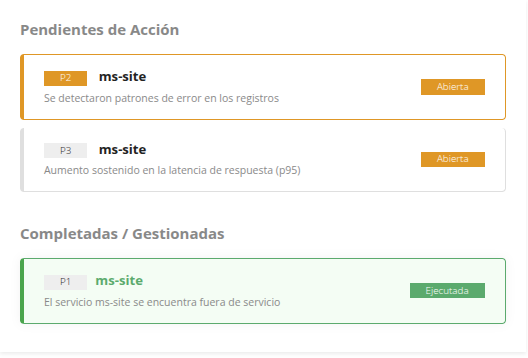
\includegraphics[width=0.9\textwidth]{graphics/paware-alerts-list.png}
    \caption{Listado de alertas autonómicas priorizadas visibles para el administrador.}
    \label{fig:paware-alerts-list}
\end{figure}
\begin{figure}[htbp]
    \centering
    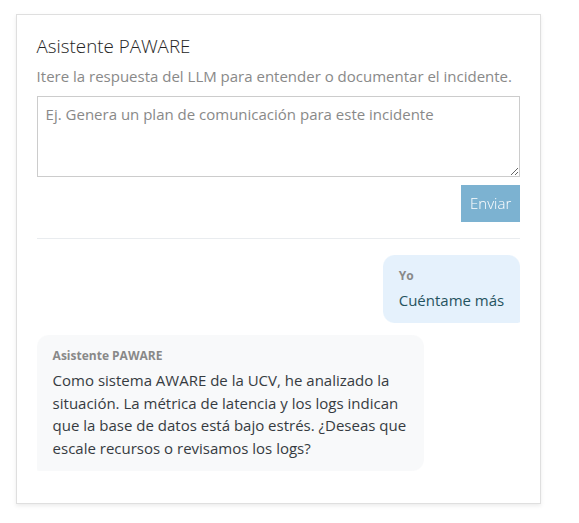
\includegraphics[width=0.9\textwidth]{graphics/paware-chat.png}
    \caption{Interacción del administrador con el agente de IA para evaluar una alerta específica.}
    \label{fig:paware-chat}
\end{figure}

